\subsection{Fisheye} \label{subsec:fisheye}

The basic principle behind a Fisheye transformation is in the creation of a map. The goal is to create a map for every pixel in the original image and then approximate the value of that pixel to a new location determined by the map. 

With a Fisheye transformation we are usually taking a square or rectangular image and converting it to a circle, with varying degrees of distortion as you approach the edge of the circle. 

Begin with an image $I_{M\times N}$. Initially, we create an array $A_{M\times N}$ with $A_{i,j}=(i,j)$. We then resize this array to be a $2\times\frac{M\cdot N}{2}$ matrix. Now, each row represents an $(x,y)$ pair. We compute the median value of this array and use it to determine the distance each $(x,y)$ pair is from the center of the image. We then have an $x$ distance and a $y$ distance for each pair. We use these as the two lines of a right triangle opposite the hypotenuse. We then apply the Pythagorean Theorem to determine the length of the radius, which is the hypotenuse of the triangle. 

After that, it is just a matter of reducing that radius and curving the edges. This is done by reducing the radii in half and normalizing for the total variance in distances. We then collapse them and use a formula that as pixels get closer to the edge they stack closer together. After that a simple use of geometric formulas produces the new $x$ and $y$ distances from the center of the image using our new radii, and we have our map. 

This map is applied with nearest neighbor interpolation to determine which pixel is taken from the original image and used in the new image.

\begin{figure}[H]
    \centering
    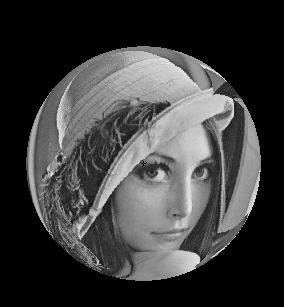
\includegraphics[scale=0.5]{images/fisheye.png}
    \caption{Fish Eye Transformation}
    \label{fig:lenna-fish-eye}
\end{figure}